\section{Simulation Analysis}
\label{sec:simulation}

\subsection{Operating Point Analysis}

Table~\ref{tab:op} shows the simulated operating point results for the circuit under analysis.

\begin{table}[htb!]
  \centering
  \begin{tabular}{|l|r|}
    \hline    
    {\bf Name} & {\bf Value [A or V]} \\ \hline
    @gb[i] & -2.48284e-04\\ \hline
@r1[i] & 2.369027e-04\\ \hline
@r2[i] & -2.48284e-04\\ \hline
@r3[i] & -1.13810e-05\\ \hline
@r4[i] & 1.210640e-03\\ \hline
@r5[i] & -2.48284e-04\\ \hline
@r6[i] & 9.737374e-04\\ \hline
@r7[i] & 9.737374e-04\\ \hline
v(1) & 5.185042e+00\\ \hline
v(2) & 4.941554e+00\\ \hline
v(3) & 4.425830e+00\\ \hline
v(5) & 4.977013e+00\\ \hline
v(6) & 5.729012e+00\\ \hline
v(7) & -1.97652e+00\\ \hline
v(8) & -2.95469e+00\\ \hline
v(9) & 0.000000e+00\\ \hline

  \end{tabular}
  \caption{Operating point results. A variable preceded by @ is of type {\em current}
    and expressed in Ampere; other variables are of type {\it voltage} and expressed in
    Volt.}
  \label{tab:op}
\end{table}

These results were produced using the \textit{Ngspice software}. In order for the \textit{software} to be able to recognise the Current-Controlled Voltage Source, defined in Figure \ref{fig2} as $H_c$, we had to add a new Independent Voltage Source with a voltage of 0V, which is also represented in \ref{fig2}.


\begin{figure}[h] \centering
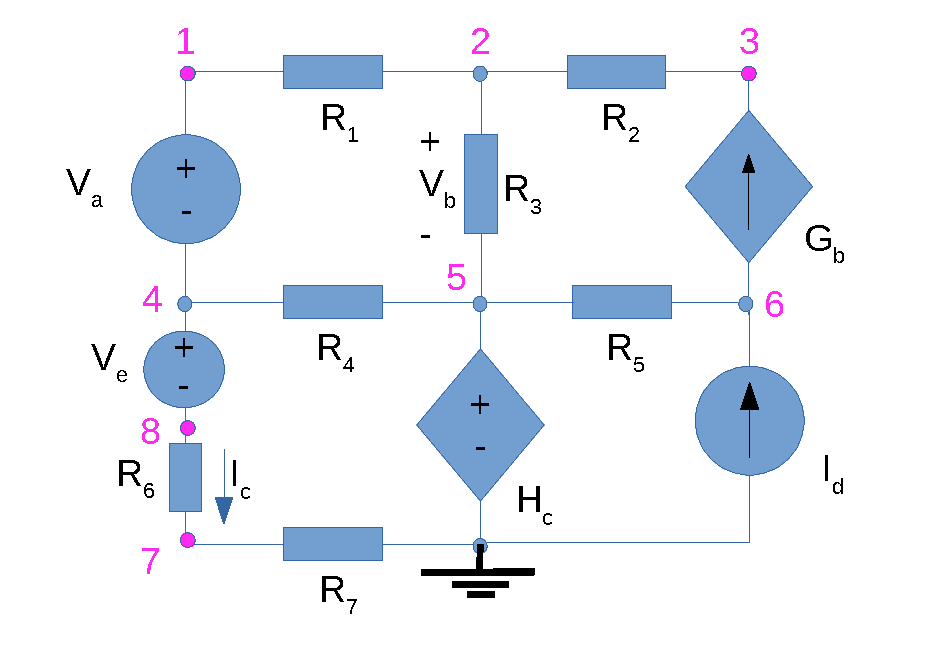
\includegraphics[width=0.4\linewidth]{t1-2.pdf}
\caption{The original circuit with an added voltage source of value 0V.}
\label{fig2}
\end{figure}